% G07 - Fase 2, Entrega final - apresentacao
\documentclass[aspectratio=169,11pt]{beamer}
\usetheme{default}
\usepackage{fontspec}
\setsansfont{TeX Gyre Heros}
\usepackage{booktabs,amsmath,tikz,array}
\usepackage{newunicodechar}
\newunicodechar{Ω}{\ensuremath{\Omega}}
\newunicodechar{→}{\ensuremath{\to}}
\newunicodechar{×}{\ensuremath{\times}}
\newunicodechar{·}{\ensuremath{\cdot}}
\newunicodechar{≈}{\ensuremath{\approx}}
\newunicodechar{≤}{\ensuremath{\le}}
\newunicodechar{°}{\ensuremath{^\circ}}
\newunicodechar{µ}{\ensuremath{\mu}}
\newunicodechar{σ}{\ensuremath{\sigma}}
\newunicodechar{−}{\ensuremath{-}}
\definecolor{az}{HTML}{1F4E8C}\definecolor{azc}{HTML}{E8F0FA}
\definecolor{vm}{HTML}{C0392B}\definecolor{cz}{HTML}{5A6270}
\setbeamercolor{normal text}{fg=black!85}
\setbeamercolor{structure}{fg=az}
\setbeamercolor{frametitle}{fg=az}
\setbeamerfont{frametitle}{size=\Large,series=\bfseries}
\setbeamertemplate{navigation symbols}{}
\setbeamertemplate{itemize item}{\color{az}\rule[0.25ex]{0.6ex}{0.6ex}}
\setbeamertemplate{frametitle}{\vspace{2pt}\insertframetitle\par\vspace{1pt}{\color{az}\rule{2.2cm}{2pt}}\vspace{-4pt}}
\setbeamertemplate{footline}{\leavevmode\hbox to\paperwidth{\hspace{12pt}\scriptsize\color{cz}\rodape\hfill\insertframenumber\hspace{12pt}}\vspace{6pt}}
\newcommand{\fig}[2][\textwidth]{\includegraphics[width=#1]{../relatorio/figuras/#2}}
\newcommand{\kpi}[3][2.55cm]{\begin{tikzpicture}\node[fill=azc,rounded corners=3pt,inner sep=6pt,text width=#1,align=center]{{\Large\bfseries\color{az}#2}\\[1pt]{\scriptsize\color{cz}#3}};\end{tikzpicture}}
\newcommand{\kpivm}[3][2.55cm]{\begin{tikzpicture}\node[fill=vm!10,rounded corners=3pt,inner sep=6pt,text width=#1,align=center]{{\Large\bfseries\color{vm}#2}\\[1pt]{\scriptsize\color{cz}#3}};\end{tikzpicture}}
\newcommand{\capa}[3]{{\setbeamertemplate{footline}{}\setbeamercolor{background canvas}{bg=az}
\begin{frame}\color{white}\vspace{1.4cm}
{\small #1}\\[10pt]{\huge\bfseries #2}\\[6pt]{\Large #3}\\[24pt]
{\color{white}\rule{3cm}{1.5pt}}\\[10pt]
\small Nícolas De Almeida Souza · Lucas Momesso Alves · Cláudio Henrique da Costa Santos
\end{frame}}}
\newcommand{\destaque}[1]{\begin{center}\colorbox{azc}{\parbox{.9\textwidth}{\centering\vspace{5pt}#1\vspace{5pt}}}\end{center}}
\newcommand{\pontos}[6]{\begin{tabular}{@{}>{\raggedright\arraybackslash}p{.3\textwidth}@{\hspace{.035\textwidth}}>{\raggedright\arraybackslash}p{.3\textwidth}@{\hspace{.035\textwidth}}>{\raggedright\arraybackslash}p{.3\textwidth}@{}}
#1 & #3 & #5\\[4pt]\small #2 & \small #4 & \small #6\end{tabular}}
\newcommand{\contexto}[1]{{\small\color{cz}#1}\par\vspace{4pt}}
\usetikzlibrary{positioning,fit,backgrounds,arrows.meta}
\newunicodechar{≪}{\ensuremath{\ll}}\newunicodechar{←}{\ensuremath{\leftarrow}}\newunicodechar{≥}{\ensuremath{\ge}}
\newcommand{\pend}{\textcolor{red}{?}}
\newcommand{\rodape}{Instrumentação não ideal e seus efeitos no controle}
\begin{document}

\capa{Fase 2 · Entrega final}{Instrumentação não ideal e seus efeitos no controle}{Corrente de fase do motor BLDC medida com o sensor Hall ACS712}

\begin{frame}{A mensagem em uma frase}
\contexto{O que o instrumento entrega ao controlador difere do que a planta realmente faz.}
\vspace{6pt}
\destaque{O mesmo PI que acerta a corrente com medição ideal deixa o motor 23 mA abaixo da referência com a medição real.}
\vspace{12pt}
\centering
\kpivm[3.05cm]{23 mA}{erro (limite 30)}\hfill
\kpivm[3.05cm]{1,4 mV}{zero que derruba}\hfill
\kpivm[3.05cm]{15 mV}{ruído que derruba}\hfill
\kpi[3.05cm]{11 mA}{erro após compensar}
\end{frame}

\begin{frame}{1 · Sistema original e analogia}
\contexto{O motor BLDC aciona um ventilador. No equivalente, a parte elétrica fica em 1:1 e a mecânica vira circuito pela analogia força–tensão.}
\centering\resizebox{.6\textwidth}{!}{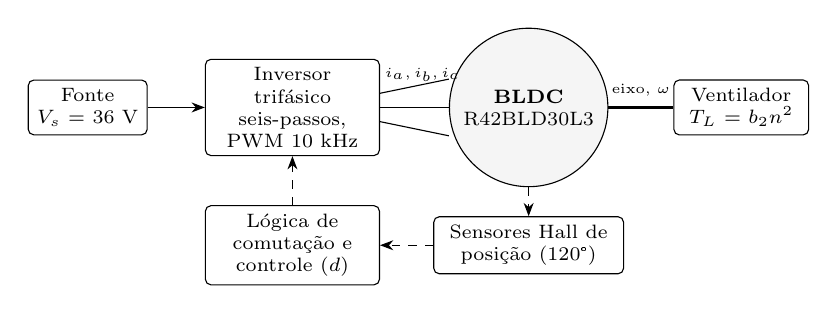
\begin{tikzpicture}[font=\scriptsize, >=Stealth, bx/.style={draw, rounded corners=2pt, align=center, fill=white, inner sep=3pt}]
\node[bx, text width=1.3cm] (vs) at (0,0) {Fonte\\$V_s$ = 36 V};
\node[bx, text width=2.0cm] (inv) at (2.6,0) {Inversor trifásico\\seis-passos, PWM 10 kHz};
\node[draw, circle, minimum size=1.55cm, align=center, fill=gray!8] (m) at (5.6,0) {\textbf{BLDC}\\R42BLD30L3};
\node[bx, text width=1.5cm] (fan) at (8.3,0) {Ventilador\\$T_L = b_2 n^2$};
\node[bx, text width=2.2cm] (hl) at (5.6,-1.75) {Sensores Hall de posição (120°)};
\node[bx, text width=2.0cm] (lg) at (2.6,-1.75) {Lógica de comutação e controle ($d$)};
\draw[->] (vs) -- (inv);
\foreach \y in {-0.18,0,0.18} \draw ([yshift=\y cm]inv.east) -- ([yshift=\y cm]m.west |- 0,\y);
\node[above, font=\tiny] at (4.25,0.2) {$i_a, i_b, i_c$};
\draw[line width=1.4pt] (m.east) -- node[above, font=\tiny]{eixo, $\omega$} (fan.west);
\draw[->, dashed] (m.south) -- (hl.north);
\draw[->, dashed] (hl) -- (lg);
\draw[->, dashed] (lg) -- (inv);
\end{tikzpicture}
}\\[4pt]
{\small $L_J\dfrac{di_m}{dt} + R_B i_m = v_{Te} - v_{carga} \;\Longleftrightarrow\; J\dfrac{d\omega}{dt} + B\omega = T_e - T_L - T_d$}\\[4pt]
\kpi[3.05cm]{100 V}{por N·m}\hfill
\kpi[3.05cm]{1 A}{= 1000 rpm}\hfill
\kpi[3.05cm]{34,56 mH}{$L_J$ (inércia)}\hfill
\kpi[3.05cm]{1:1}{corrente e tempo}
\end{frame}

\begin{frame}{1 · Circuito equivalente no TyphoonSim}
\contexto{Fase $a$ (b e c iguais): em cima, o lado elétrico do motor; embaixo, a malha mecânica com $L_J$, $R_B$ e as fontes de torque.}
\centering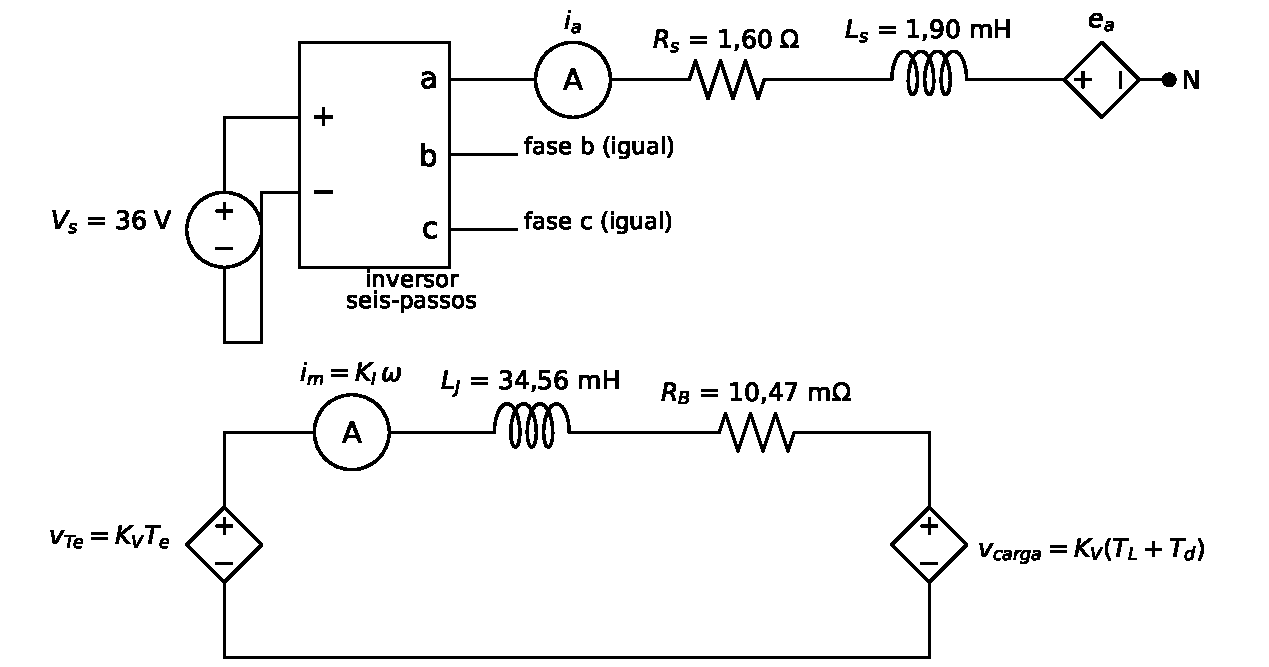
\includegraphics[width=.97\textwidth,height=.68\textheight,keepaspectratio]{../relatorio/figuras/fig_circuito.pdf}
\end{frame}

\begin{frame}{2 · Onde atua a instrumentação}
\contexto{A Figura 1 da orientação com os blocos do modelo. O sensor lê o amperímetro ideal de cada fase; o seletor escolhe o que chega ao PI.}
\centering\resizebox{!}{.71\textheight}{% Figura 1 da orientacao, preenchida com os blocos do modelo_final.tse (G07)
\begin{tikzpicture}[font=\scriptsize, >=Stealth,
  bx/.style={draw, rounded corners=2pt, align=center, fill=white, inner sep=3pt, text width=#1},
  bx/.default=2.5cm,
  ins/.style={bx=#1, fill=gray!10}, ins/.default=2.5cm]
\node[bx=2.6cm] (pl) at (0,0) {\textbf{Planta}\\(equivalente elétrico)\\[1pt]{\tiny fases \texttt{G07\_Rs/Ls/e\_x};\\ mecânica \texttt{G07\_L\_J}, \texttt{G07\_R\_B}}};
\node[bx=2.7cm] (pp) at (3.7,0) {\textbf{Ponta de prova ideal}\\[1pt]{\tiny \texttt{G07\_iS}, \texttt{G07\_iSb}: amperímetros em série com as fases a e b}};
\node[bx=2.9cm] (id) at (7.6,1.75) {\textbf{Caminho ideal}: ganho 1\\[1pt]{\tiny \texttt{G07\_Med\_ideal}; $i_{pl}$ em \texttt{G07\_CL\_realimentacao}}};
\node[bx=2.3cm] (sel) at (11.0,0) {\textbf{Seletor ideal/real}\\[1pt]{\tiny caixa \texttt{G07\_fb\_real}}};
\node[bx=2.4cm] (rf) at (15.2,1.75) {\textbf{Referência} $r$\\[1pt]{\tiny \texttt{G07\_CL\_referencia}}};
\node[bx=2.4cm] (ct) at (15.2,0) {\textbf{Controlador}\\[1pt]{\tiny \texttt{G07\_CL\_erro} (Sum) e \texttt{G07\_CL\_PI} (PI)}};
\node[bx=2.4cm] (at) at (15.2,-2.45) {\textbf{Atuador}\\[1pt]{\tiny \texttt{G07\_Seletor\_duty} e inversor (PWM 10 kHz)}};
\node[ins=2.45cm] (se) at (4.9,-2.45) {\textbf{Sensor} ACS712-20A\\[1pt]{\tiny \texttt{S1} sensibilidade · \texttt{S2} zero\\ \texttt{S3} banda · \texttt{S4} ruído}};
\node[ins=2.45cm] (co) at (7.85,-2.45) {\textbf{Condicionamento}\\[1pt]{\tiny \texttt{C1} filtro RC 15 kHz\\ \texttt{C2} ADC 12 bits, 20 kS/s}};
\node[ins=2.75cm] (pr) at (10.95,-2.45) {\textbf{Processamento e compensação}\\[1pt]{\tiny \texttt{P1}: correção calculada, média, autocalibração; \texttt{CL\_realimentacao}: módulo ou Hall, correção do RC}};
\begin{scope}[on background layer]
\node[draw=gray, dashed, rounded corners, fill=gray!4, fit=(se)(co)(pr), inner sep=5pt] (box) {};
\end{scope}
\node[font=\scriptsize\bfseries, above=0pt of box.north] {Aqui atua a instrumentação (cadeias das fases a e b)};
\node[bx=3.6cm] (es) at (7.85,-4.55) {\textbf{Entradas espúrias}\\[1pt]{\tiny temperatura (\texttt{G07\_T} = 60 °C); ruído e interferência (\texttt{G07\_ruido})}};
\draw[->] (pl) -- node[above]{$y_{real}$} (pp);
\draw[->] (pp.east) -- ++(0.35,0) |- (id.west);
\draw[->] (pp.south) |- (se.west);
\draw[->] (se) -- (co); \draw[->] (co) -- (pr);
\draw[->] (id.east) -| (sel.north);
\draw[->] (pr.north) -- (pr.north |- sel.south);
\draw[->] (sel) -- node[above, font=\tiny, align=center]{$y_{ideal}$\\ou $y_{med}$} (ct);
\draw[->] (rf) -- (ct); \draw[->] (ct) -- (at);
\draw[->] (es) -- (box.south -| es);
\draw[->, dashed] ([xshift=-6mm]box.south) |- (0.4,-3.75) node[pos=0.75, below, font=\tiny, align=center]{carregamento: 1,2 m$\Omega$ ≪ 1,6 $\Omega$ (< 0,04 \%), desprezado} -- ([xshift=4mm]pl.south);
\draw[->] (at.south) -- ++(0,-2.55) -| node[pos=0.25, below, font=\tiny]{ação de controle: razão cíclica $d$ (atuador → planta)} ([xshift=-4mm]pl.south);
\end{tikzpicture}
}
\end{frame}

\begin{frame}{2 · Sensor escolhido: Hall ACS712-20A}
\contexto{A grandeza é a corrente de fase, que produz o torque ($T = k\,i$). Os requisitos vêm da corrente simulada do motor.}
\begin{columns}[c]
\column{.5\textwidth}
\begin{itemize}\setlength{\itemsep}{8pt}\small
\item Mais simples que o shunt: \textbf{isolado} e já com \textbf{saída em tensão}
\item Ramo medido: fases a e b, em série com $R_s$, $L_s$, $e_x$; escala 1:1
\item $i_c = -(i_a + i_b)$, sem terceiro sensor
\item Carregamento: 1,2 m$\Omega$ contra 1,6 $\Omega$, menos de 0,04 \%: desprezado
\end{itemize}
\column{.46\textwidth}\centering\footnotesize
\renewcommand{\arraystretch}{1.25}
\begin{tabular}{@{}lll@{}}\toprule
 & \textbf{Demanda} & \textbf{ACS712 + cadeia}\\\midrule
Faixa & ±10 A & ±25 A\\
Banda & 3,5 kHz & 80 kHz\\
Resolução & 40 mA & 12 mA\\
Viés & 25 mA & ≤ 2 mA\\
Aleatório & 70 mA & 58 mA\\
Atraso & 100 µs & 60 µs\\\bottomrule
\end{tabular}
\end{columns}
\end{frame}

\begin{frame}{3 · Características do instrumento}
\contexto{Cada uma é um bloco do caminho real, ajustável no SCADA, com valor do datasheet ou estimativa declarada.}
\centering\scriptsize
\renewcommand{\arraystretch}{1.22}
\begin{tabular}{@{}llll@{}}\toprule
\textbf{Característica} & \textbf{Tipo (livro)} & \textbf{Valor} & \textbf{Efeito esperado na leitura}\\\midrule
Desvio de zero & estática (3.3.8) & +10 mV & +100 mA constantes\\
Erro de sensibilidade & estática (3.3.1) & +1,5 \% & escala 1,5 \% maior\\
Temperatura & espúria (2.4) & 60 °C & zero $-$2,45 mV; ganho $-$0,14 \%\\
Resposta do sensor & dinâmica (4.2.2) & 80 kHz & atraso de 2 µs\\
Ruído & espúria (5.4) & 10 mV rms & 100 mA rms (34 mA após filtrar)\\
Filtro RC & \textbf{circuito auxiliar} (6.2.1) & 15 kHz & atenua $f_e$ se $f_c$ for baixo\\
ADC & \textbf{circuito auxiliar} (3.3.2) & 12 bits, 20 kS/s & degrau de 12 mA; retenção 50 µs\\
Média por período & \textbf{processamento} (6.2.2) & 100 µs & tira os 10 kHz; atraso de 50 µs\\
Módulo $|i_a|+|i_b|+|i_c|$ & \textbf{processamento} & — & retifica o ruído: +14 mA\\\bottomrule
\end{tabular}
\end{frame}

\begin{frame}{4 · Em malha aberta: cada característica isolada}
\contexto{Cada bloco também calcula a leitura só com a sua característica. Uma captura separa as contribuições.}
\fig[.84\textwidth]{fig_contribuicoes.pdf}\\[4pt]
\kpivm[3.05cm]{75,5 mA}{zero sem correção}\hfill
\kpi[3.05cm]{1,2 mA}{zero com correção}\hfill
\kpi[3.05cm]{58 mA}{erro rms (limite 70)}\hfill
\kpi[3.05cm]{60 µs}{atraso (limite 100)}
\end{frame}

\begin{frame}{5 · Controle com instrumento ideal}
\contexto{PI nativo, projetado cancelando o polo elétrico ($K_p$ = 0,264; $K_i$ = 222). O seletor realimenta a corrente verdadeira.}
\vspace{4pt}\centering\small
\renewcommand{\arraystretch}{1.35}
\begin{tabular}{@{}lcc@{}}\toprule
\textbf{Critério} & \textbf{Limite} & \textbf{Medição ideal}\\\midrule
Erro estacionário & ≤ 30 mA & \textbf{9 mA}\\
Acomodação (±5 \%) & ≤ 3 ms & \textbf{1,4 ms}\\
Sobressinal & ≤ 10 \% & \textbf{5 \%}\\
Esforço: desvio de $d$ & ≤ 0,08 & \textbf{0,047}\\
Afundamento de 10 \% & ≤ 0,30 A & \textbf{0,17 A}\\\bottomrule
\end{tabular}
\vspace{10pt}
\destaque{Com medição ideal, todos os critérios são atendidos.}
\end{frame}

\begin{frame}{6 · Mesmo controle, instrumento real}
\contexto{Só o seletor muda. A medida chega a 1,500 A, mas a corrente verdadeira fica abaixo, e a acomodação passa a falhar.}
\begin{columns}[c]
\column{.62\textwidth}\fig{fig_r3.pdf}
\column{.34\textwidth}\centering
\kpi[3.1cm]{1,500 A}{medida (realimentada)}\\[5pt]
\kpivm[3.1cm]{1,478 A}{planta (verdadeira)}\\[5pt]
\kpivm[3.1cm]{4,8 ms}{acomodação (limite 3)}
\end{columns}
\end{frame}

\begin{frame}{6 · Quem causa cada diferença}
\contexto{Cada diferença entre ideal e real volta para uma característica da Tab. 3.}
\vspace{4pt}
\begin{itemize}\setlength{\itemsep}{9pt}\small
\item \textbf{Erro de 23 mA na planta} ← \textbf{ruído} retificado pelo \textbf{módulo}: na fase sem corrente, $|n|$ tem média $\sigma\sqrt{2/\pi}$; ≈ +14 mA na medida (+5 mA da amostragem do ADC), e o PI reduz a corrente real
\item \textbf{Acomodação 1,4 → 4,8 ms (falha)} ← o mesmo viés: a planta assenta perto da borda da faixa de 5 \%
\item \textbf{Sobressinal 5 → 6 \%, queda 0,17 → 0,20 A} ← \textbf{atraso} de 60 µs (média, ADC, RC): margem de fase 83° → 74°
\item \textbf{Esforço igual} ← a \textbf{média por período} tira os 10 kHz da realimentação
\item \textbf{Sem efeito}: zero, ganho e temperatura, porque a \textbf{correção calculada} usa os valores calibrados
\end{itemize}
\end{frame}

\begin{frame}{7 · Ponto de ruptura}
\contexto{Cada característica varrida em 4 níveis numa só captura. As previsões foram registradas antes de simular.}
\vspace{2pt}\centering\small
\renewcommand{\arraystretch}{1.35}
\begin{tabular}{@{}lccc@{}}\toprule
\textbf{Característica} & \textbf{Previsão} & \textbf{Ruptura (erro)} & \textbf{Por quê}\\\midrule
Zero não compensado & 1,2 mV & \textbf{1,4 mV} & planta = $i^* - \frac23\delta$\\
Ruído & 19 mV & \textbf{15 mV} & viés $0{,}455\,\sigma_f$\\
Filtro RC & 1,2 kHz & \textbf{0,95 kHz} & planta = $i^*/|H(f_e)|$\\\bottomrule
\end{tabular}
\vspace{12pt}
\destaque{1,4 mV é menos que a deriva térmica do próprio sensor (2,45 mV a 60 °C).}
\end{frame}

\begin{frame}{8 · Compensações do Cap. 2}
\contexto{Duas das três rupturas nascem no circuito auxiliar: no filtro RC (analógico) e no módulo (processamento digital).}
\vspace{4pt}
\pontos{{\color{az}\large\bfseries Ruído retificado}}{\textbf{Insensibilidade inerente} (2.5.1): usa a fase em condução indicada pelos sensores Hall de posição, sem módulo.}{{\color{az}\large\bfseries Zero}}{\textbf{Correção calculada} com autocalibração (2.5.3): 5 ms com o inversor parado na partida.}{{\color{vm}\large\bfseries Filtro RC}}{\textbf{Correção calculada} (2.5.3): divide a medida por $|H(f_e)|$, com $f_e$ do Hall.}
\vspace{14pt}
\kpi[3.05cm]{15 → 78 mV}{ruptura do ruído}\hfill
\kpi[3.05cm]{1,4 → 97 mV}{ruptura do zero}\hfill
\kpivm[3.05cm]{1,7 kHz}{ruptura do RC (era 0,96: piorou)}\hfill
\kpi[3.05cm]{23 → 11 mA}{erro na planta}
\end{frame}

\begin{frame}{8 · Resultados, contra as previsões}
\contexto{Previsões registradas antes das capturas: a do ruído se confirmou; a do filtro RC, não.}
\fig[.88\textwidth]{fig_item8_erro.pdf}\\[2pt]
\begin{columns}[T]
\column{.48\textwidth}\footnotesize
\textbf{Ruído:} sem retificação, o erro só falha com 78 mV. O limite global vai a 17 mV (previsto 19): passa a ser o sobressinal, que é aleatório.
\column{.48\textwidth}\footnotesize
\textbf{RC:} a medida pela posição lê a fase depois que o filtro assentou; $|H(f_e)|$ não vale, e a correção piora em 1 kHz. Melhor exigir $f_c$ ≥ 1,2 kHz.
\end{columns}
\end{frame}

\begin{frame}{9 · O que exigir de cada parte}
\contexto{Em malha fechada, o que desloca a média da leitura passa inteiro para o motor; o que só a espalha é atenuado.}
\vspace{8pt}
\pontos{{\color{vm}\Large\bfseries Sensor}}{Zero calibrado no sistema (a deriva passa de 1,4 mV); ruído ≤ 15–17 mV rms; banda de 80 kHz não limita.}{{\color{az}\Large\bfseries Condicionamento}}{RC com $f_c$ ≥ 1,2 kHz (corrigir não substitui); ADC 12 bits síncrono com o PWM.}{{\color{az}\Large\bfseries Processamento}}{Correção calculada, média por período, autocalibração e fase pela posição.}
\vspace{18pt}
\destaque{O instrumento é decisivo pelo viés, não pela velocidade.}
\end{frame}

\end{document}
